\documentclass[12pt,a4paper]{article}

% =================================================
% Font (XeLaTeX or LuaLaTeX REQUIRED)
% =================================================
\usepackage{fontspec}
\setmainfont{Trebuchet MS}

\usepackage{listings}
\usepackage{xcolor}
\usepackage{subcaption}

\lstset{
    language=Python,
    basicstyle=\ttfamily\small,
    keywordstyle=\color{blue},
    stringstyle=\color{red},
    commentstyle=\color{gray},
    showstringspaces=false,
    breaklines=true,
    frame=single
}

% =================================================
% Math and symbols
% =================================================
\usepackage{amsmath,amssymb,amsfonts}

% =================================================
% Graphics and floats
% =================================================
\usepackage{graphicx}
\usepackage{float}
\usepackage{placeins}

\usepackage{hanging}
\usepackage{ragged2e}

% =================================================
% Tables
% =================================================
\usepackage{booktabs}
\usepackage{multirow}

% =================================================
% Lists and layout
% =================================================
\usepackage{enumitem}
\usepackage{geometry}
\geometry{margin=1in}

% =================================================
% TOC customization
% =================================================
\usepackage[titles]{tocloft}
\renewcommand{\cftsecleader}{\cftdotfill{\cftdotsep}}

% =================================================
% Citations
% =================================================
\usepackage{cite}

% =================================================
% Hyperlinks (no colors, no boxes)
% =================================================
\usepackage[hidelinks]{hyperref}

% =================================================
% Title (UNCHANGED AS REQUESTED)
% =================================================
\title{
\textbf{Pilot Study Report}\\[0.5em]
Adaptive Multi-LLM Agentic RAG with Dynamic Task Routing and Retrieval Planning
}

\author{Partha Pratim Mazumder}
\date{}

% =================================================
% Document Begins
% =================================================
\begin{document}

% ---------------- Custom Title Page ----------------
\begin{titlepage}
    \centering
    
    % University logo
    
\includegraphics[width=0.3\textwidth]{../assets/solent_logo.png}\\[0.8cm]
    
    {\LARGE \textbf{SOLENT UNIVERSITY SOUTHAMPTON}}\\[0.4cm]
    {\large Department of Science and Engineering}
    
    \vspace{1.5cm}
    
    {\Large \textbf{Dissertation - Research Project (COM726)}}\\[0.4cm]
    {\large \textbf{Pilot Study Report}}\\[0.2cm]
    {\small \textbf{Academic Year 2025--2026}}
    
    \vspace{1.5cm}
    
    % ===== Your Preserved Title =====
    {\Huge \textbf{Adaptive Multi-LLM Agentic RAG}}\\[0.3cm]
    {\Large \textbf{with Dynamic Task Routing and Retrieval Planning}}
    
    \vspace{1.5cm}
    
    {\Large \textbf{Partha Pratim Mazumder}}\\[0.2cm]
    {\large Student ID: Q103063737}\\[0.1cm]
    {\small \texttt{0mazup37@solent.ac.uk}}
    
    \vspace{1.2cm}
    
    {\large \textbf{Module Leader: Dr Bacha Rehman}}\\[0.3cm]
    {\large \textbf{Submission Date: \today}}
    
    \vspace{0.8cm}
    
    {\footnotesize \copyright~Solent University, \the\year}
    
\end{titlepage}

% =================================================
% Front Matter
% =================================================
\pagenumbering{roman}
\tableofcontents
\newpage

% =================================================
% Main Content
% =================================================
\pagenumbering{arabic}


% =================================================
\section{Introduction}

Recent advances in large language models (LLMs) have enabled powerful conversational systems capable of reasoning, code generation, and knowledge-intensive question answering. However, most deployed systems rely on monolithic architectures in which a single model is responsible for handling all user queries, regardless of task complexity or reasoning requirements. This approach often leads to inefficiencies, unnecessary retrieval overhead, increased hallucination risk, and suboptimal resource utilisation.

This pilot study proposes an adaptive conversational AI framework that dynamically routes user queries to specialised LLMs, tools, and retrieval pipelines based on inferred task intent and complexity. Rather than invoking retrieval-augmented generation (RAG) or agentic reasoning by default, the system selectively activates these components only when they provide measurable benefits.

\subsection{Problem Definition}

Static RAG pipelines and always-on agentic systems introduce avoidable latency, token consumption, and system complexity. Many user queries can be answered directly using parametric model knowledge, while others require specialised reasoning or structured retrieval. The absence of intelligent routing mechanisms limits scalability and robustness in real-world deployments.

\subsection{Research Context and Motivation}

Emerging frameworks such as ReAct and LangGraph demonstrate the potential of tool-augmented reasoning, yet they often assume persistent agentic execution. This research is motivated by the need for a lightweight, production-oriented alternative that balances intelligence, efficiency, and reliability.

\subsection{Structure of the Report}

This report presents the background and justification for the proposed research, defines the research aim and objectives, describes the proposed artefact and its societal impact, and evaluates the feasibility of implementation through a structured project plan.

\section{Literature Review}

Retrieval-Augmented Generation (RAG) enhances Large Language Models (LLMs) by grounding responses in external 
knowledge sources, reducing hallucination and knowledge staleness (Singh et al., 2025). Early retrieve-then-generate 
pipelines relied on sparse retrieval methods such as BM25, but subsequent advances introduced dense retrieval, 
modular architectures, and graph-based reasoning to improve semantic alignment and multi-hop performance 
(Singh et al., 2025). Agentic RAG extends this paradigm by embedding autonomous agents capable of planning, tool 
use, reflection, and adaptive retrieval. Dynamic orchestration frameworks such as MAO-ARAG enable cost-aware workflow planning through multi-agent coordination (Chen et al., 2025), while MA-RAG emphasizes collaborative reasoning without additional training (Nguyen et al., 2025). Structured reasoning and tool integration have been advanced through ART and AutoTool, which enable programmatic reasoning and dynamic tool selection (Paranjape et al., 2023; Zou et al., 2025). Planning-driven approaches such as PAR-RAG incorporate complexity-aware decomposition and verification mechanisms to enhance factual consistency (Zhang et al., 2025), and RAG-Gym introduces systematic optimization through actor–critic training and process-level supervision (Xiong et al., 2025). Despite these advances, challenges remain in scalable multi-agent coordination, adaptive multi-LLM specialization, robust verification, and cost–latency trade-offs, motivating adaptive multi-LLM agentic RAG architectures.


\section{Research Aim, Objectives, and Questions}

\subsection{Research Aim}

The aim of this research is to design and evaluate an adaptive multi-LLM conversational system that improves reasoning accuracy, efficiency, and robustness through dynamic task routing and selective retrieval planning.

\subsection{Research Objectives}

\begin{itemize}
    \item Design an intent-aware routing mechanism for query classification.
    \item Implement specialist LLM delegation for reasoning and coding tasks.
    \item Develop an adaptive RAG pipeline with retrieval necessity prediction.
    \item Evaluate agentic execution only for complex multi-step queries.
    \item Compare efficiency and accuracy against static single-model baselines.
\end{itemize}

\subsection{Research Questions}

\begin{enumerate}
    \item How accurately can a routing agent determine whether a query requires retrieval, specialised reasoning, or direct inference?
    \item Does delegating tasks to specialist LLMs outperform single-model approaches?
    \item Can adaptive retrieval planning reduce hallucinations and computational overhead?
    \item When does agentic reasoning provide measurable benefits over direct generation?
    \item How does routing performance vary across different reasoning domains?
\end{enumerate}

% =================================================

\section{Proposed Artefact and Societal Impact}

\subsection{Description of the Proposed Artefact}

The proposed artefact is a modular conversational AI system built using a multi-LLM architecture with dynamic routing, adaptive RAG, and optional agentic execution, implemented using LangGraph-style state management.

\subsection{Technical Scope}

The system integrates intent classifiers, specialist language models, vector databases, and execution controllers to enable conditional tool use.

\subsection{Societal and Industry Impact}

The artefact contributes to safer and more efficient AI systems by reducing hallucinations, lowering operational costs, and improving response reliability in knowledge-critical applications such as education, research assistance, and enterprise support.

\subsection{Relevance to Computing Discipline}

This project demonstrates advanced computing concepts including distributed AI systems, optimisation trade-offs, state management, and applied machine learning.

% =================================================

\section{Project Resources and Feasibility Analysis}

\subsection{Required Resources}

\begin{itemize}
    \item Python programming environment
    \item LLM APIs and open-source models
    \item Vector databases (e.g., FAISS)
    \item Benchmark datasets: HotpotQA, ChronoQA, MuSiQue
\end{itemize}

\subsection{Data Requirements}

Publicly available datasets will be used exclusively, minimising ethical concerns.

\subsection{Ethical Considerations}

No personal or sensitive data will be processed. The project aligns with institutional ethics policies.

\subsection{Risk Assessment}

Potential risks include model latency and integration complexity, mitigated through modular design.


\section{Project Implementation Plan}


\subsection{Methodology Overview}

The project adopts a modular and iterative methodology centered around an adaptive orchestration pipeline. 
User queries are processed through a unified interface and persisted via checkpointed state management. 
A central orchestration layer dynamically routes each query based on its inferred requirements, enabling 
direct response generation, adaptive document retrieval, or agent-based multi-step execution. 
This design allows controlled experimentation across routing, retrieval, and agentic reasoning strategies 
while maintaining a consistent system backbone.

\subsection{System Architecture Flow}

Figure~\ref{fig:system_flowchart} illustrates the high-level execution flow of the system. 
The architecture begins with user interaction and state persistence, followed by query processing 
and adaptive routing. Depending on the routing decision, queries may invoke retrieval, agent planning 
with tool execution, or direct response generation, all of which converge through a unified task 
execution layer before producing the final response.

\begin{figure}[htbp]
    \centering
    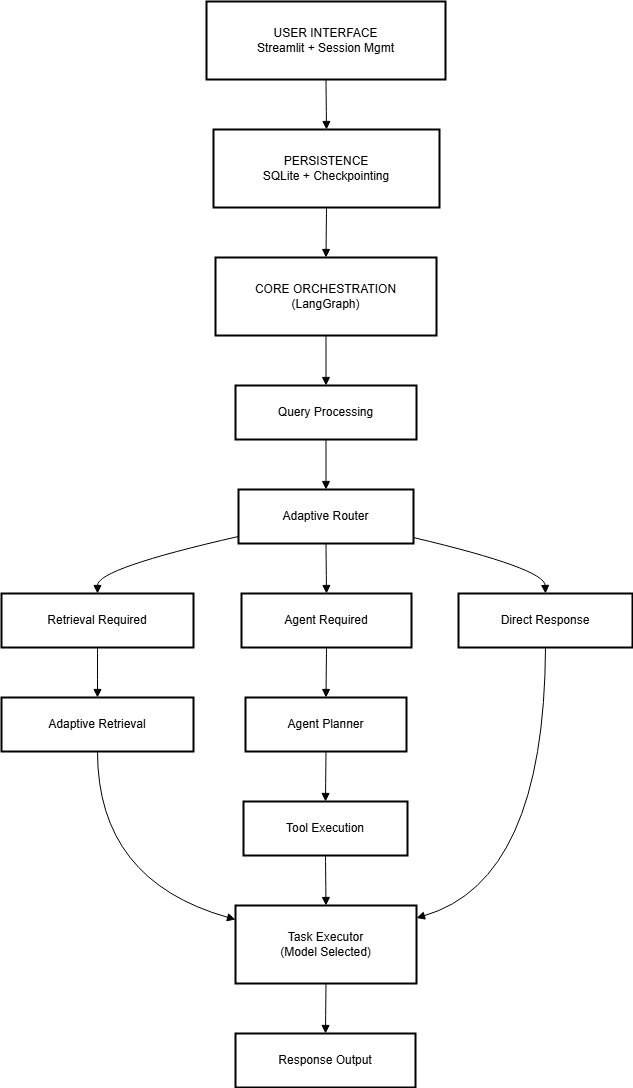
\includegraphics[
        width=0.9\linewidth,
        height=0.6\textheight,
        keepaspectratio
    ]{../assets/flowchart.png}
    \caption{High-level system flowchart illustrating adaptive routing, retrieval, and agent execution.}
    \label{fig:system_flowchart}
\end{figure}

Figure~\ref{fig:system_ui} presents the current implementation of the system’s user interface. 
The interface serves as the primary interaction layer through which user queries are submitted 
and responses are rendered, integrating seamlessly with the underlying orchestration and 
state management pipeline.

\begin{figure}[htbp]
    \centering
    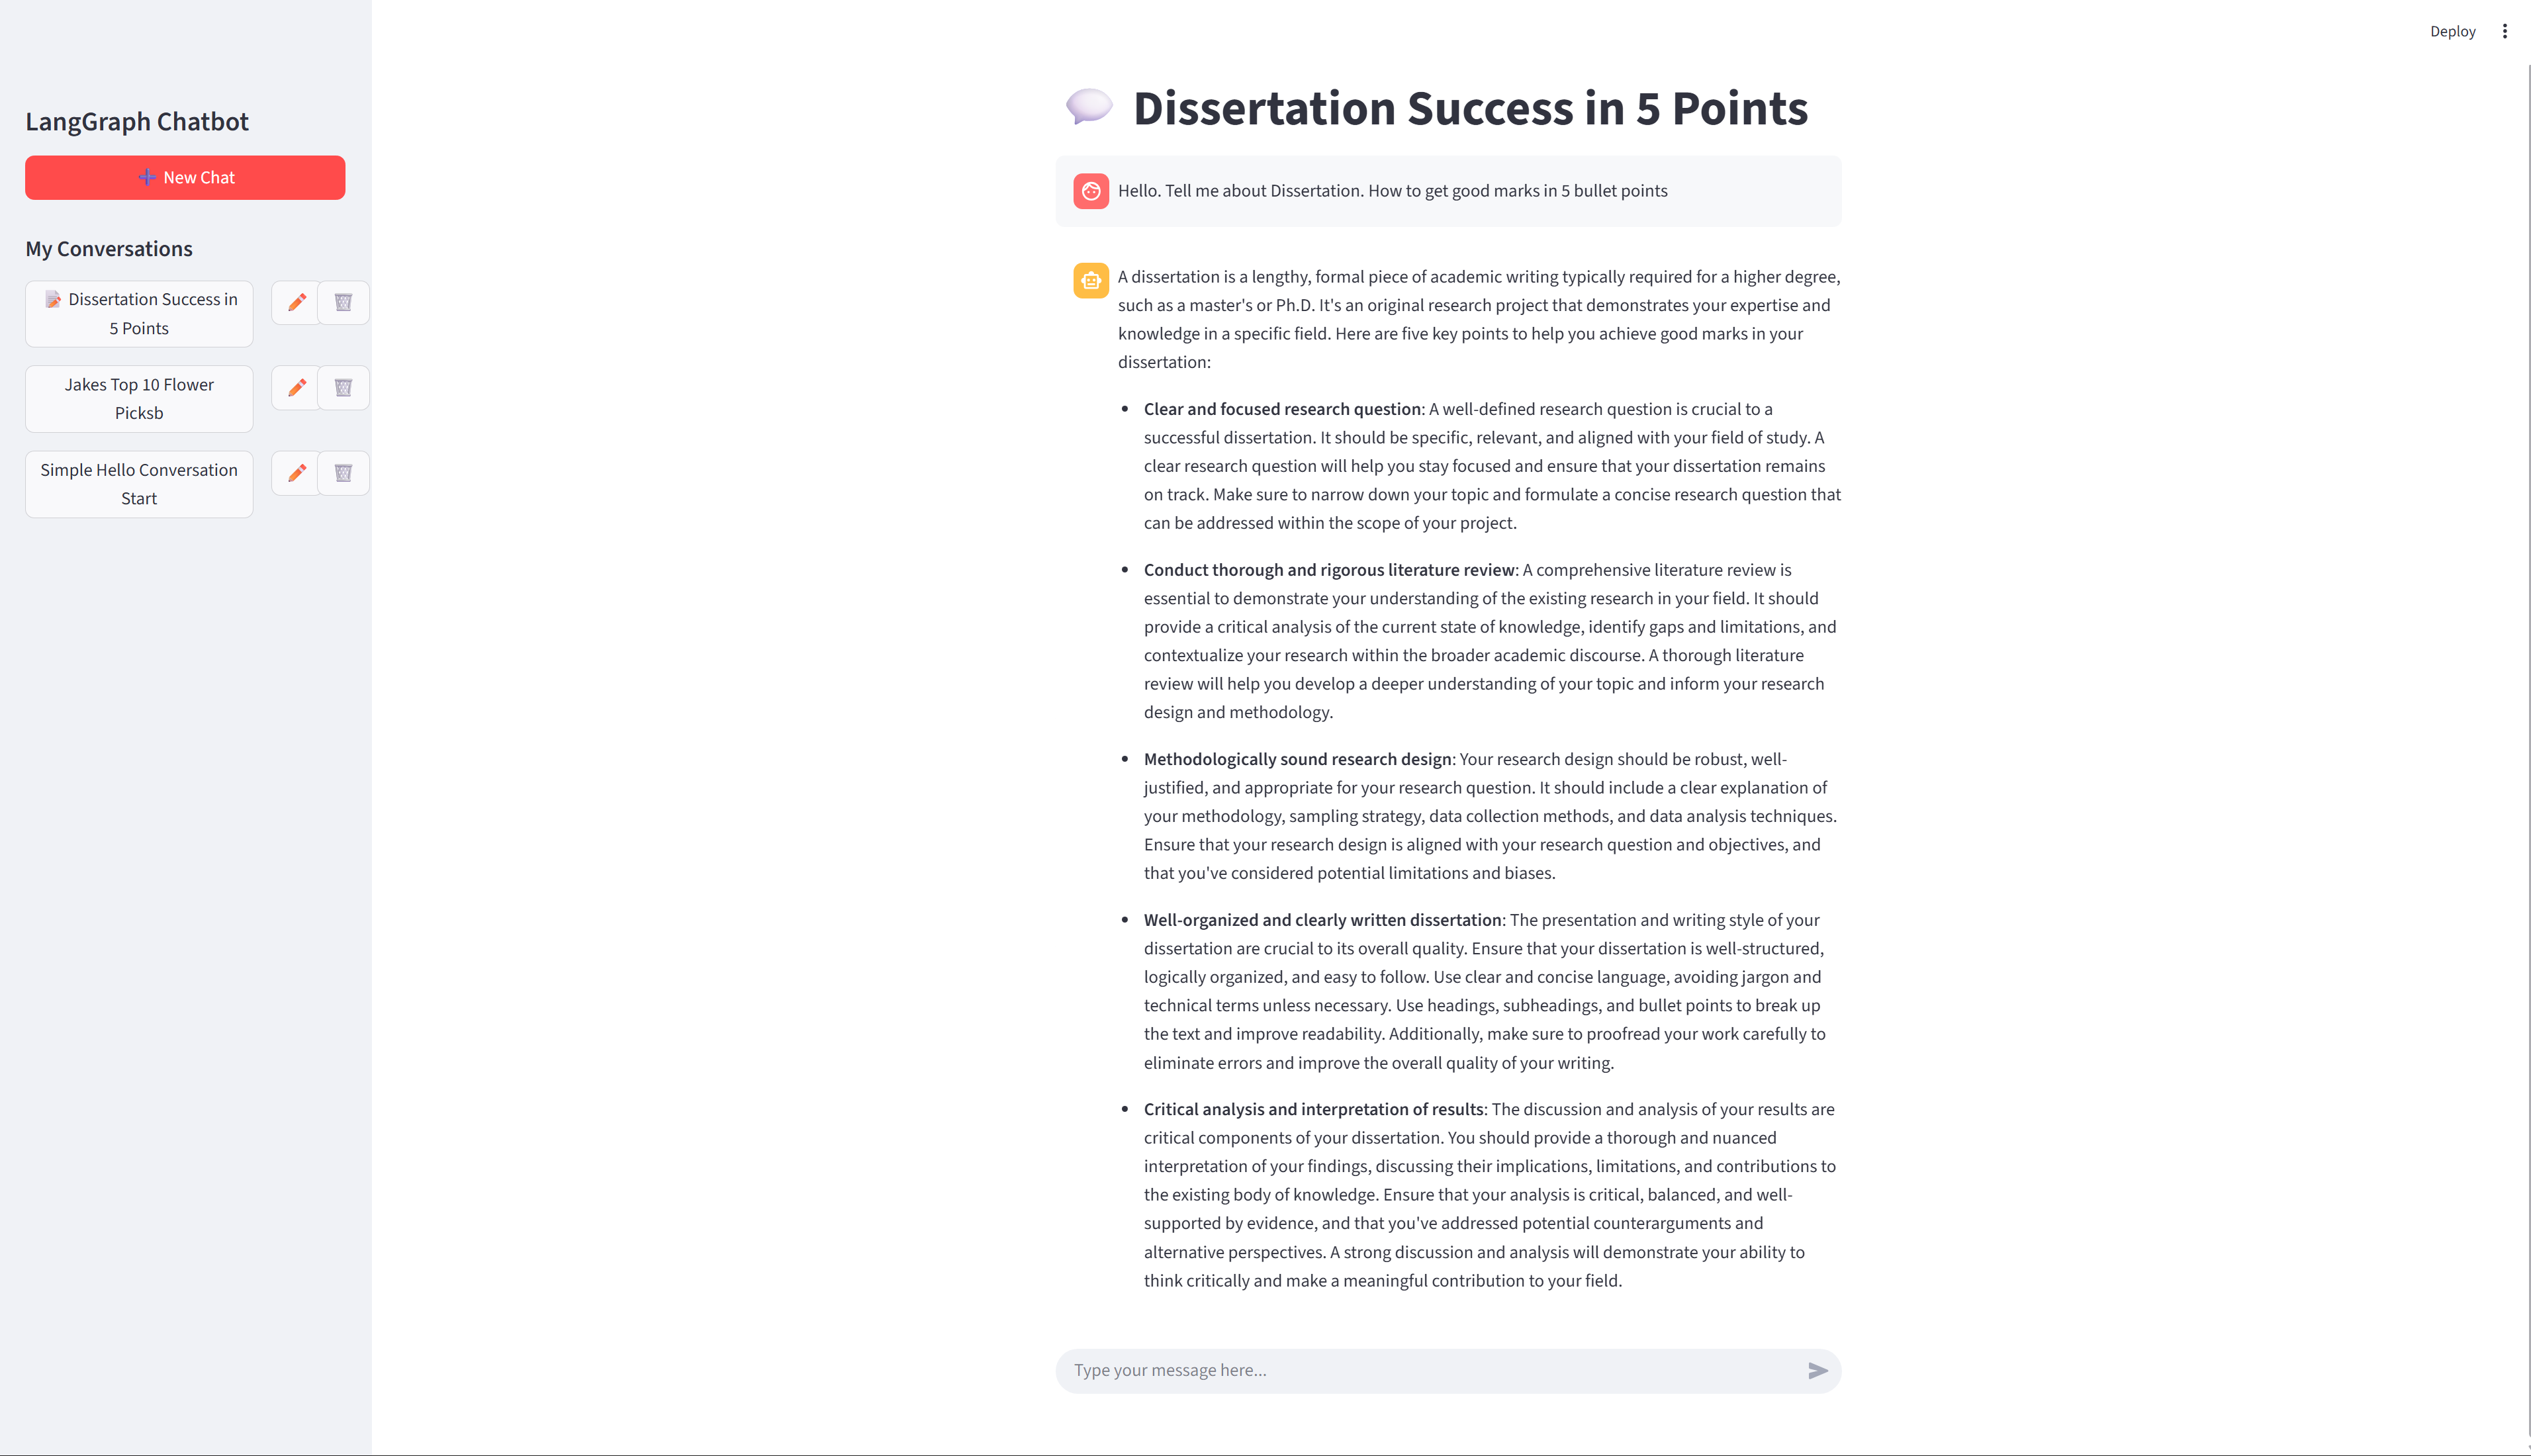
\includegraphics[
        width=0.9\linewidth,
        height=0.6\textheight,
        keepaspectratio
    ]{../assets/ui.png}
    \caption{Current implementation of the system user interface integrated with the adaptive orchestration pipeline.}
    \label{fig:system_ui}
\end{figure}

\FloatBarrier

\subsection{Project Timeline}

The project is scheduled over a multi-phase timeline spanning from mid-January to early May 2026. 
The implementation progresses through four structured stages. The initial phase focuses on research 
and planning, including literature review, dataset selection, and foundational learning of retrieval 
and orchestration frameworks. This is followed by a core system execution phase, where the baseline 
system, persistence layer, adaptive routing logic, retrieval components, and agent execution mechanisms 
are incrementally implemented.

Subsequent stages emphasize system integration and experimental evaluation, including hallucination 
analysis, routing accuracy assessment, and comparative benchmarking across different execution paths. 
The final phase is dedicated to documentation, result consolidation, and preparation of the final 
report, ensuring that experimental findings are clearly articulated and reproducible.

\subsection{Gantt Chart}

The complete project schedule, including task dependencies, parallel development tracks, and milestone 
deliverables, is presented in the Gantt chart provided in Figure ~\ref{fig:gantt_chart}. The chart captures the temporal 
distribution of activities across research, system development, evaluation, and reporting phases, 
spanning the full project duration from January 17, 2026 to May 2, 2026.

\begin{figure}[htbp]
    \centering
    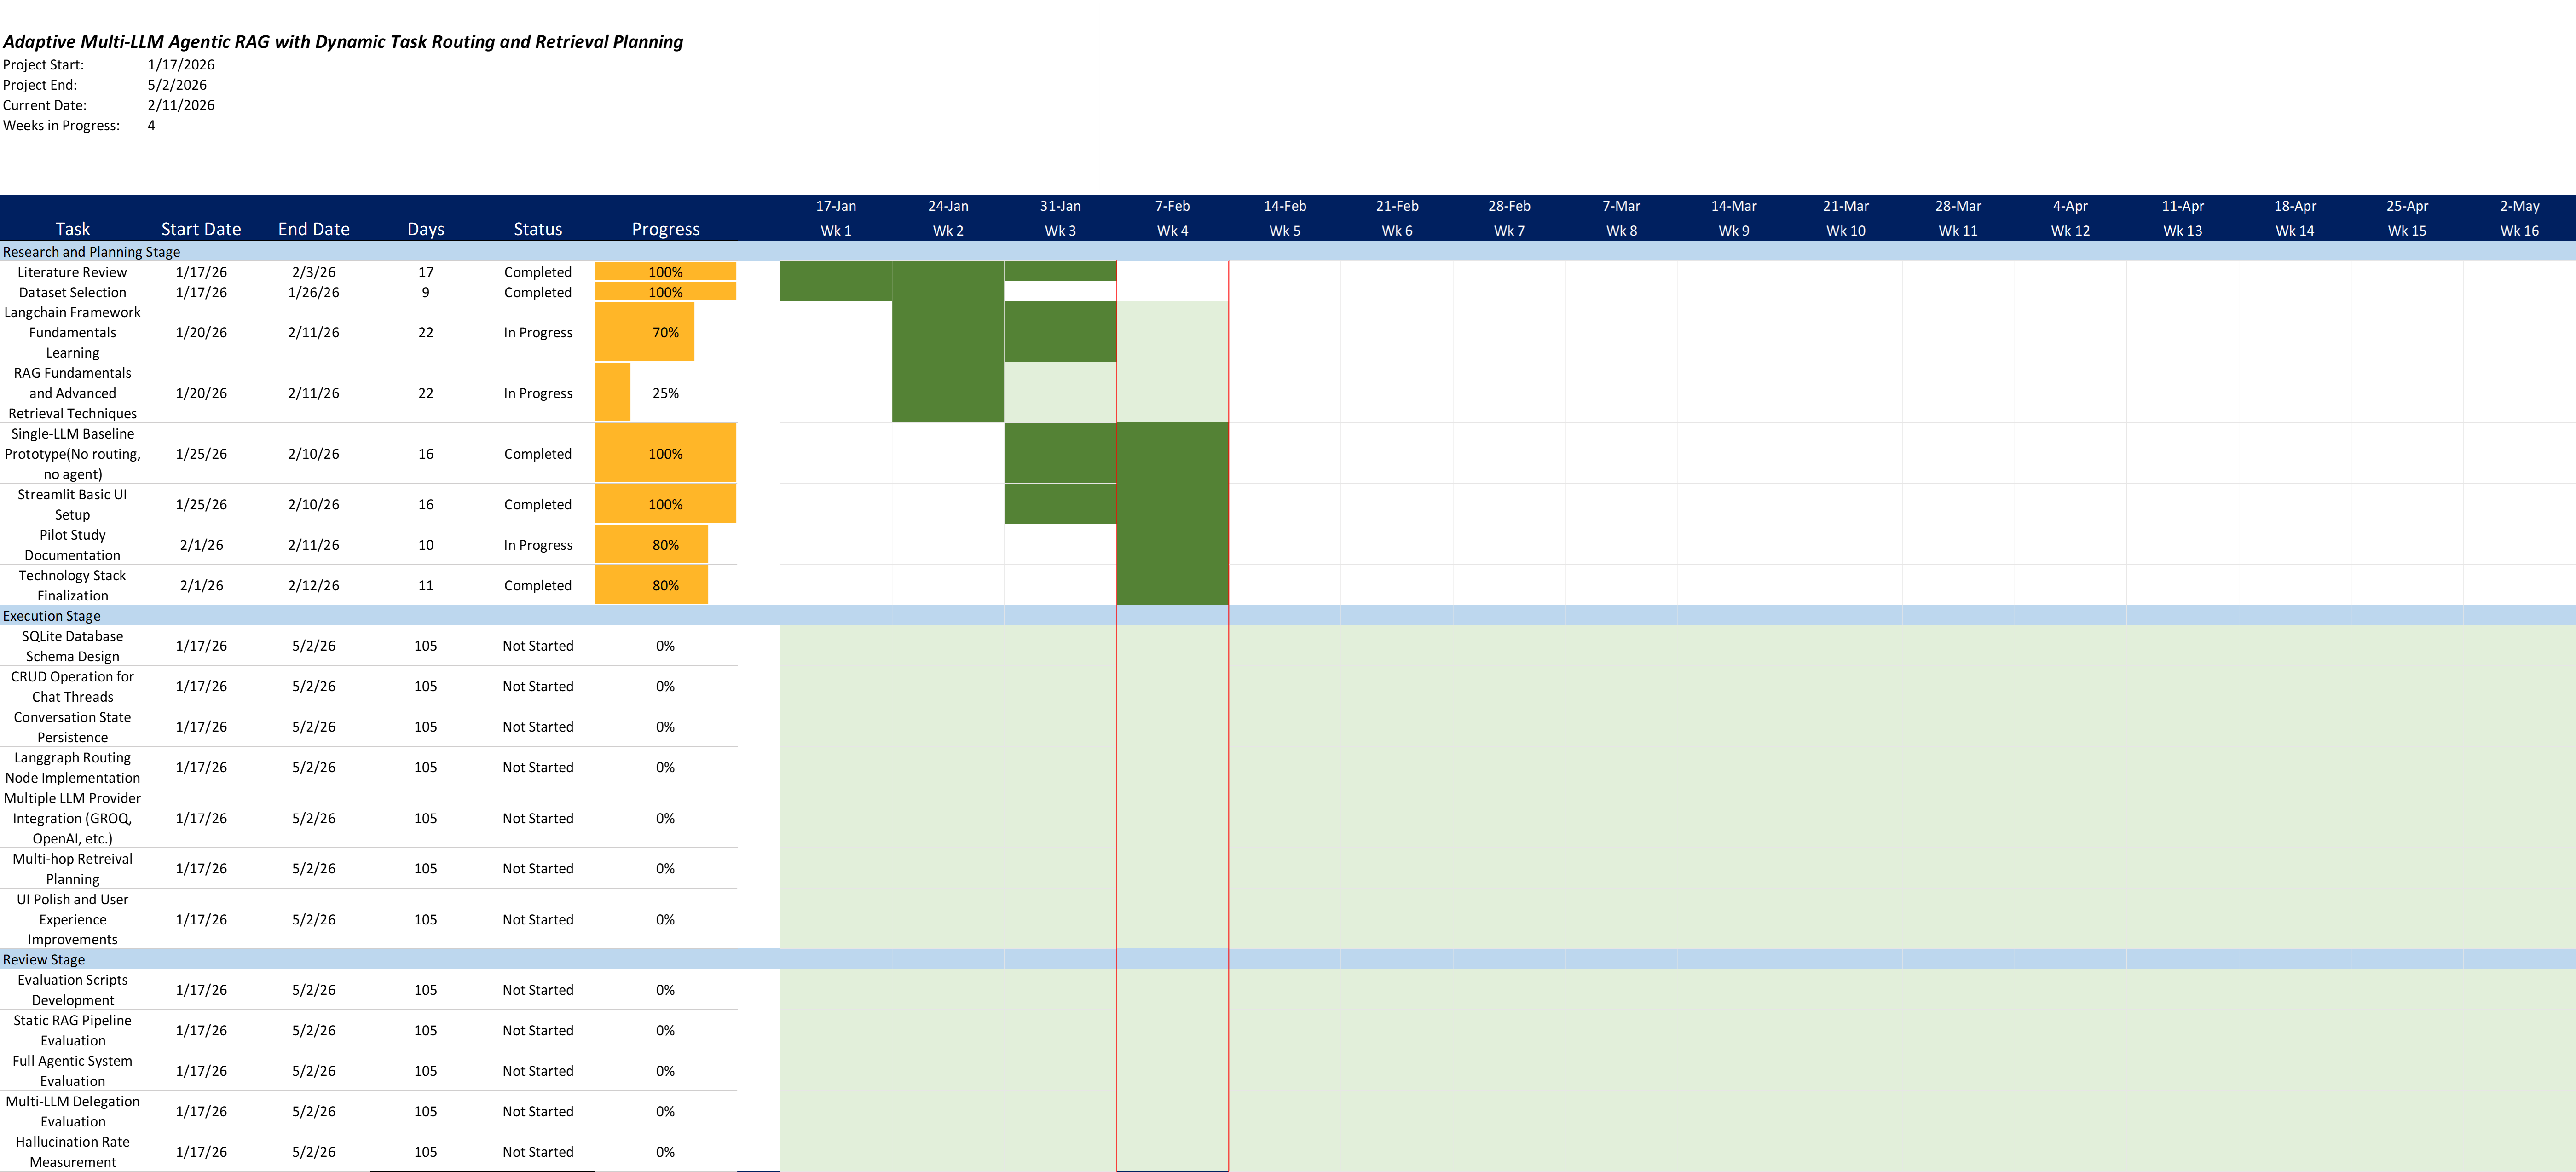
\includegraphics[width=\textwidth]{../assets/gnatt_chart.png}
    \caption{Project Gantt Chart illustrating the full project timeline from January 17, 2026 to May 2, 2026.}
    \label{fig:gantt_chart}
\end{figure}

\FloatBarrier


\newpage

\section{Conclusion}

This pilot study demonstrates the feasibility and academic value of an adaptive multi-LLM conversational framework. The proposed approach addresses key limitations in static RAG and agentic systems by introducing dynamic task routing, modular orchestration, and controlled experimentation across retrieval and reasoning strategies. By integrating adaptive routing with retrieval augmentation and agent-based execution, the framework enables more context-aware, scalable, and flexible response generation.

The study establishes a structured architectural foundation that supports comparative evaluation of direct generation, retrieval-enhanced responses, and multi-step agentic reasoning within a unified system backbone. This modular design not only facilitates systematic experimentation but also enhances reproducibility and extensibility for future research.

Overall, the pilot validates the technical viability of the proposed system and provides a clear roadmap for the full MSc dissertation project, where deeper empirical evaluation, quantitative benchmarking, and comprehensive analysis of routing effectiveness, hallucination mitigation, and performance trade-offs will be conducted.

\newpage

\section*{References}
\addcontentsline{toc}{section}{References}

\setlength{\parindent}{0pt}
\setlength{\parskip}{0.8em}

\justifying
\sloppy

CHEN, Y., ZHANG, E., YAN, L., WANG, S., HUANG, J., YIN, D. and MAO, J., 2025. 
MAO-ARAG: Multi-Agent Orchestration for Adaptive Retrieval-Augmented Generation. 
\textit{arXiv preprint arXiv:2508.01005}. 
Available from: 
\url{https://arxiv.org/abs/2508.01005}

NGUYEN, T., CHIN, P. and TAI, Y.-W., 2025. 
MA-RAG: Multi-Agent Retrieval-Augmented Generation via Collaborative Chain-of-Thought Reasoning. 
\textit{arXiv preprint arXiv:2505.20096}. 
Available from: 
\url{https://arxiv.org/abs/2505.20096}

PARANJAPE, B., LUNDBERG, S., SINGH, S., HAJISHIRZI, H., ZETTLEMOYER, L. and RIBEIRO, M.T., 2023. 
ART: Automatic multi-step reasoning and tool-use for large language models. 
\textit{arXiv preprint arXiv:2303.09014}. 
Available from: 
\url{https://arxiv.org/abs/2303.09014}

SINGH, A., EHTESHAM, A., KUMAR, S. and TALAEI KHOEI, T., 2025. 
Agentic Retrieval-Augmented Generation: A survey on Agentic RAG. 
\textit{arXiv preprint arXiv:2501.09136}. 
Available from: 
\url{https://arxiv.org/abs/2501.09136}

XIONG, G., JIN, Q., WANG, X., FANG, Y., LIU, H., YANG, Y., CHEN, F., SONG, Z., WANG, D., ZHANG, M., LU, Z. and ZHANG, A., 2025. 
RAG-Gym: Systematic Optimization of Language Agents for Retrieval-Augmented Generation. 
\textit{arXiv preprint arXiv:2502.13957}. 
Available from: 
\url{https://arxiv.org/abs/2502.13957}

ZHANG, N., ZHANG, C., TAN, Z., YANG, X., DENG, W. and WANG, W., 2025. 
Credible plan-driven RAG method for multi-hop question answering. 
\textit{arXiv preprint arXiv:2504.16787}. 
Available from: 
\url{https://arxiv.org/abs/2504.16787}

ZOU, J., YANG, L., QI, Y., CHEN, S., AI, M., SHEN, K., HE, J. and WANG, M., 2025. 
AutoTool: Dynamic tool selection and integration for agentic reasoning. 
\textit{arXiv preprint arXiv:2508.xxxxx}. 
Available from: 
\url{https://arxiv.org/abs/2508.xxxxx}


% =================================================
\appendix

\end{document}
